\documentclass[12pt]{article}
\usepackage[a4paper,margin=1.25cm]{geometry}
\usepackage{amsmath,amssymb,mathtools}
\usepackage{graphicx}
\usepackage{booktabs}
\usepackage{tabularx}
\usepackage{tikz}
\usetikzlibrary{angles,quotes}
\usepackage[T1]{fontenc}
\usepackage[utf8]{inputenc}
\usepackage[english]{babel}

\setlength{\parindent}{0pt}
\setlength{\parskip}{0.45em}
\setlength{\abovedisplayskip}{5pt plus 1pt minus 1pt}
\setlength{\belowdisplayskip}{5pt plus 1pt minus 1pt}
\setlength{\abovedisplayshortskip}{3pt plus 1pt minus 1pt}
\setlength{\belowdisplayshortskip}{3pt plus 1pt minus 1pt}

\newcommand{\dd}{\,\mathrm{d}}
\newcommand{\ii}{\mathrm{i}}
\newcommand{\e}{\mathrm{e}}
\newcommand{\ang}{^\circ}
\newcommand{\Gam}{\Gamma}

\begin{document}

\begin{center}
{\Large\bfseries Two \(60\ang\) angles, an isosceles cevian, and a hidden circle}\\[0.35em]
{\large the invariant \(AD-BD=DE\), then the power of a point}
\end{center}

\textbf{Problem.} In triangle \(ABC\), the point \(D\) lies on side
\(BC\) and the point \(E\) lies on side \(AC\). Suppose
\[
AD=DC,\qquad BD=8,\qquad DE=7,\qquad
\angle BAC=\angle ADE=60\ang .
\]
Find \(AB\).

\[
\boxed{\displaystyle AB=\frac{161}{13}.}
\]

\textbf{Overview.}
The solution has two independent halves, and each one produces an
integer.

The first half determines \(AD\). Setting \(\alpha=\angle DAC\), the
isosceles condition \(AD=DC\) makes \(\angle ADB=2\alpha\), and the two
triangles \(ABD\) and \(AED\) turn out to share the angle
\(120\ang-\alpha\) opposite to \(AD\). The sine rule in each then gives
\(AD\) and \(BD\) as multiples of \(DE\), and the difference collapses by
a sum-to-product identity:
\[
AD-BD=DE\cdot\frac{\sin(120\ang-\alpha)-\sin(60\ang-\alpha)}{\sin\alpha}
=DE .
\]
So \(AD=BD+DE=8+7=15\), independently of \(\alpha\).

The second half uses the circle \(\Gam\) centred at \(D\) with radius
\(AD=15\). Both \(A\) and \(C\) lie on it. Let \(P\) be the second
intersection of line \(AB\) with \(\Gam\). The inscribed angle
\(\angle PAC=60\ang\) gives the central angle \(\angle PDC=120\ang\),
hence \(\angle PDB=60\ang\); the law of cosines in triangle \(PDB\)
returns \(PB=13\); and the power of the point \(B\) with respect to
\(\Gam\) gives
\[
AB\cdot PB=(AD-BD)(AD+BD)=7\cdot23=161 .
\]

\section*{1. The configuration}

\begin{center}
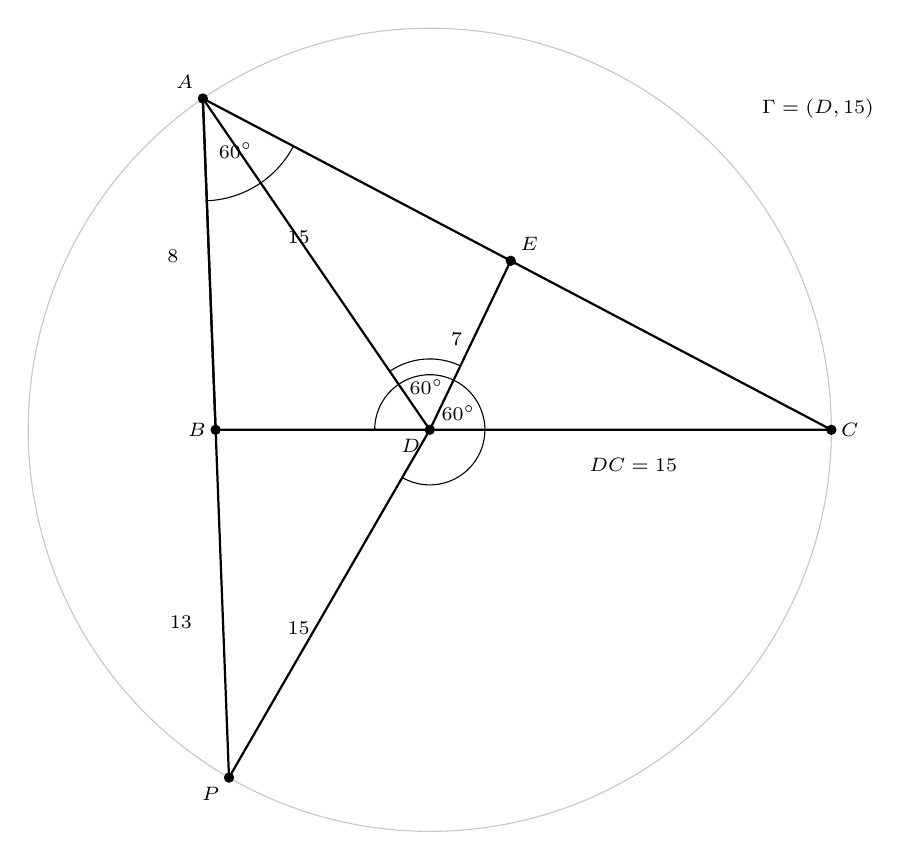
\begin{tikzpicture}[scale=0.34,>=stealth]
\coordinate (D) at (0,0);
\coordinate (B) at (-8,0);
\coordinate (C) at (15,0);
\coordinate (A) at (-8.4763,12.3755);
\coordinate (E) at (3.0237,6.3133);
\coordinate (P) at (-7.5,-12.9904);

\draw[gray!45] (D) circle (15);

\draw[thick] (A)--(B)--(C)--cycle;
\draw[thick] (A)--(D);
\draw[thick] (D)--(E);
\draw[thick] (A)--(P);
\draw[thick] (D)--(P);

\fill (A) circle (5.5pt) node[above left] {\scriptsize \(A\)};
\fill (B) circle (5.5pt) node[left] {\scriptsize \(B\)};
\fill (C) circle (5.5pt) node[right] {\scriptsize \(C\)};
\fill (D) circle (5.5pt) node[below left] {\scriptsize \(D\)};
\fill (E) circle (5.5pt) node[above right] {\scriptsize \(E\)};
\fill (P) circle (5.5pt) node[below left] {\scriptsize \(P\)};

\node at (-9.6,6.5) {\scriptsize \(8\)};
\node at (-4.9,7.2) {\scriptsize \(15\)};
\node at (1.0,3.4) {\scriptsize \(7\)};
\node at (7.6,-1.3) {\scriptsize \(DC=15\)};
\node at (-4.9,-7.4) {\scriptsize \(15\)};
\node at (-9.3,-7.2) {\scriptsize \(13\)};

\pic[draw,angle radius=13mm,"\scriptsize \(60\ang\)"]{angle=B--A--C};
\pic[draw,angle radius=9mm,"\scriptsize \(60\ang\)"]{angle=E--D--A};
\pic[draw,angle radius=7mm,"\scriptsize \(60\ang\)"]{angle=P--D--B};
\node at (14.5,12) {\scriptsize \(\Gam=(D,15)\)};
\end{tikzpicture}
\end{center}

Write \(\alpha=\angle DAC\). The data are
\[
AD=DC,\qquad BD=8,\qquad DE=7,\qquad
\angle BAC=\angle ADE=60\ang,
\]
with \(B,D,C\) collinear in that order and \(E\) on segment \(AC\).

\textbf{Angle chase.}
\begin{itemize}
\item Triangle \(ADC\) is isosceles with \(AD=DC\), so
\(\angle ACD=\angle DAC=\alpha\).
\item \(\angle ADB\) is the exterior angle of triangle \(ADC\) at \(D\),
hence
\[
\angle ADB=\angle DAC+\angle ACD=2\alpha .
\tag{1}
\]
\item Since \(E\) lies on \(AC\), the ray \(AE\) is the ray \(AC\), so
\(\angle DAE=\angle DAC=\alpha\), and \(\angle BAD=60\ang-\alpha\).
\item In triangle \(ADE\), with \(\angle ADE=60\ang\),
\[
\angle AED=180\ang-60\ang-\alpha=120\ang-\alpha .
\tag{2}
\]
\item In triangle \(ABD\), with (1),
\[
\angle ABD=180\ang-\angle ADB-\angle BAD
=180\ang-2\alpha-(60\ang-\alpha)=120\ang-\alpha .
\tag{3}
\]
\end{itemize}

Comparing (2) and (3):
\[
\boxed{\displaystyle \angle ABD=\angle AED=120\ang-\alpha .}
\tag{4}
\]
In both triangles \(ABD\) and
\(AED\) the side \(AD\) is opposite an angle of the same size, so the two
sine rules share a common ratio.

\section*{2. The invariant \(AD-BD=DE\)}

Apply the sine rule in triangle \(ABD\) and in triangle \(AED\), using
(4):
\[
\frac{AD}{\sin\angle ABD}=\frac{BD}{\sin\angle BAD},
\qquad
\frac{AD}{\sin\angle AED}=\frac{DE}{\sin\angle DAE},
\]
that is,
\[
\frac{AD}{\sin(120\ang-\alpha)}
=\frac{BD}{\sin(60\ang-\alpha)}
=\frac{DE}{\sin\alpha}.
\tag{5}
\]
Hence
\[
AD=DE\cdot\frac{\sin(120\ang-\alpha)}{\sin\alpha},
\qquad
BD=DE\cdot\frac{\sin(60\ang-\alpha)}{\sin\alpha},
\]
and, by the sum-to-product identity
\(\sin U-\sin V=2\cos\frac{U+V}{2}\sin\frac{U-V}{2}\) with
\(U=120\ang-\alpha\), \(V=60\ang-\alpha\),
\[
\sin(120\ang-\alpha)-\sin(60\ang-\alpha)
=2\cos(90\ang-\alpha)\sin 30\ang
=\sin\alpha .
\]
Therefore
\[
\boxed{\displaystyle
AD-BD=DE\cdot\frac{\sin\alpha}{\sin\alpha}=DE .}
\tag{6}
\]
The parameter \(\alpha\) has cancelled completely: (6) is a relation
among the three lengths alone, valid for every admissible configuration.
With the given data,
\[
AD=BD+DE=8+7=15,
\qquad DC=AD=15,\qquad BC=23 .
\tag{7}
\]

(For the record, \(\alpha\) is in fact pinned down by the data: (5) gives
\(7\sin(60\ang-\alpha)=8\sin\alpha\), i.e.
\(\tan\alpha=\frac{7\sin60\ang}{8+7\cos60\ang}\), so
\(\alpha=27.7958\ang\). It is simply never needed.)

\section*{3. The hidden circle and the point \(P\)}

Let
\[
\Gam=\text{circle centred }D\text{ of radius }AD=15 .
\]
By (7) both \(A\) and \(C\) lie on \(\Gam\). Let \(P\) be the second
intersection of line \(AB\) with \(\Gam\).

Since \(P\), \(A\), \(C\) all lie on \(\Gam\) and \(B\) lies on segment
\(AP\), the inscribed angle at \(A\) subtending the arc \(PC\) is
\[
\angle PAC=\angle BAC=60\ang ,
\]
so the corresponding central angle is
\[
\angle PDC=2\cdot60\ang=120\ang .
\tag{8}
\]
Because \(B\), \(D\), \(C\) are collinear, the rays \(DB\) and \(DC\) are
opposite, whence
\[
\angle PDB=180\ang-120\ang=60\ang .
\tag{9}
\]

Now the law of cosines in triangle \(PDB\), with \(PD=15\), \(BD=8\) and
the included angle (9):
\[
PB^2=PD^2+BD^2-2\cdot PD\cdot BD\cos60\ang
=225+64-15\cdot8=169,
\]
so
\[
\boxed{\displaystyle PB=13 .}
\tag{10}
\]
The appearance of a Pythagorean-looking integer is not an accident; see
Section 5.

\section*{4. The power of the point \(B\)}

The point \(B\) lies inside \(\Gam\), since \(BD=8<15\). Its power with
respect to \(\Gam\) has absolute value
\[
|{\rm pow}_\Gam(B)|=AD^2-BD^2=(AD-BD)(AD+BD)=7\cdot23=161 .
\tag{11}
\]
Since the line through \(B\) meets \(\Gam\) at \(A\) and \(P\), the
intersecting-chords theorem gives
\[
AB\cdot PB=161 .
\]
With (10),
\[
AB=\frac{161}{13}=12.384615\ldots
\]

Note that (11) is expressed entirely through the invariant (6): the two
factors are \(AD-BD=DE=7\) and \(AD+BD=DE+2BD=23\). So the final answer
is a function of \(BD\) and \(DE\) alone,
\[
\boxed{\displaystyle
AB=\frac{DE\,(DE+2\,BD)}{PB},
\qquad
PB=\sqrt{(BD+DE)^2-BD(BD+DE)+BD^2}. }
\]

\section*{5. Solution B: the Eisenstein norm}

Step (10) can be recognised rather than computed. Let
\(\omega=\e^{2\pi\ii/3}\) and let
\[
N(a+b\omega)=(a+b\omega)\overline{(a+b\omega)}=a^2-ab+b^2
\]
be the norm on the ring of Eisenstein integers \(\mathbb Z[\omega]\).
Geometrically, \(N\) is exactly the squared third side of a triangle with
sides \(a\), \(b\) and included angle \(60\ang\), which is what the law
of cosines computes in (10). Hence
\[
PB^2=N(15+8\omega)=15^2-15\cdot8+8^2=225-120+64=169=13^2 .
\]

This explains the integrality. The norm form \(a^2-ab+b^2\) is
multiplicative, and its values are exactly the Loeschian numbers; that
\(N(15+8\omega)\) is a perfect square is the statement that
\((15,8,13)\) is an ``Eisenstein triple'', the \(60\ang\) analogue of a
Pythagorean triple. The problem was clearly designed around this triple:
the data \(BD=8\), \(DE=7\) were chosen so that \(AD=15\) and
\(15^2-15\cdot8+8^2\) is a square.

\begin{center}
\small
\renewcommand{\arraystretch}{1.35}
\begin{tabularx}{0.92\textwidth}{@{}lXX@{}}
\toprule
\((a,b)\) & \(N(a+b\omega)=a^2-ab+b^2\) & \(60\ang\)-triple? \\
\midrule
\((15,8)\)  & \(169=13^2\)  & yes, the one used here \\
\((8,3)\)   & \(49=7^2\)    & yes \\
\((5,3)\)   & \(19\)        & no \\
\((7,5)\)   & \(39\)        & no \\
\((16,5)\)  & \(201\)       & no \\
\((35,11)\) & \(961=31^2\)  & yes \\
\bottomrule
\end{tabularx}
\end{center}

\section*{6. What the solution used and what it did not}

\textbf{The two \(60\ang\) angles play different roles.} The angle
\(\angle ADE=60\ang\) is used only in Section 2, to produce
\(\angle AED=120\ang-\alpha\) and hence the coincidence (4). The angle
\(\angle BAC=60\ang\) is used only in Section 3, to convert an inscribed
angle into the central angle \(120\ang\). Neither is used twice.

\textbf{The isosceles condition is what creates the circle.} \(AD=DC\)
does two jobs: it gives the exterior-angle relation (1), and it places
\(C\) on the circle \(\Gam\) centred at \(D\) through \(A\). Without it
there is no natural circle in the picture, and the power-of-a-point step
would have nothing to act on.

\textbf{\(\alpha\) is never computed.} Both halves of the solution are
\(\alpha\)-free: (6) because of the sum-to-product cancellation, and
Sections 3--4 because they involve only lengths and the angle
\(\angle PDB=60\ang\). This is the structural reason the answer is a
clean rational number even though the configuration itself involves
\(\alpha=27.7958\ang\), an angle with no closed form worth writing.

\textbf{Consistency check.} Placing \(D=(0,0)\), \(B=(-8,0)\),
\(C=(15,0)\) and \(A=15(\cos(180\ang-2\alpha),\sin(180\ang-2\alpha))
=(-8.47633,12.37545)\) with \(\alpha=27.79577\ang\), one computes
\[
\angle BAC=60.0000\ang,\quad
E=(3.02367,6.31327)\in AC,\quad
DE=7.0000,\quad \angle ADE=60.0000\ang,
\]
\[
P=(-7.5,-12.99038),\quad PD=15,\quad PB=13,\quad
AB=12.3846154=\tfrac{161}{13},
\]
confirming every step numerically.

\end{document}
